% ICEA 2026 — 2026-08-07 大改版全篇重寫
%
% 改版三條指示：資料探勘反應器導向、聚焦微正壓循環裝置、大幅減少 edge 與操作史。
% ⚠ 頁數上限 10 頁（含表、圖、附錄、參考文獻）——CFP 明載 "4-6 up to 10 page"。
%   先前記載的 11 頁／10.99 係 2026-08-12 自行「定案」之誤，2026-08-23 更正。
%
% ⚠ 寫作紅線（見結構文件的「可寫／不可寫」表）：
%   · 三個統計方法全是先前技術，一律寫成 "we apply X in the sense of [cite]"
%   · 不得宣稱 r_b(k) 的函數形式、r_max、K、"mass-transfer limited"
%   · 不得寫成「已證明是生物速率」——只證明「純物理產生不出這個成分」
%   · 不得寫成模擬器已充分——殘餘 AUC 0.695
%
% 本機無 LaTeX toolchain，無法編譯驗證；改用 lint_tex.py 做靜態檢查，
% 並刻意避開 siunitx 等需要編譯才能確認的套件，單位改用自訂巨集。

\documentclass[runningheads]{llncs}

\usepackage{graphicx}
\usepackage{amsmath}
\usepackage{mhchem}
\usepackage{booktabs}
\usepackage{algorithm}
\usepackage{algpseudocode}
\usepackage[hidelinks]{hyperref}

% 單位巨集：一律用斜線式（kg/cm²、/hr），全篇統一，不用負指數。
\newcommand{\pu}{\ensuremath{\mathrm{kg/cm^{2}}}}
\newcommand{\ratu}{\ensuremath{\mathrm{kg/cm^{2}/hr}}}
\newcommand{\invh}{\ensuremath{\mathrm{/hr}}}
\newcommand{\rb}{\ensuremath{r_{b}}}
\newcommand{\rbh}{\ensuremath{\hat{r}_{b}}}
\newcommand{\kh}{\ensuremath{\hat{k}}}

\begin{document}

\title{Threshold-Triggered Cycles as Endogenous Relaxation
Experiments: Mining a Biological Methanation Rate from Quantized
Pressure}

\titlerunning{Mining a Biological Methanation Rate from Quantized Pressure}

\author{Cheng-Yu Li\inst{1} \and
Chun-Hao Chen\inst{1} \and
Cheng-Yuan Hung\inst{2} \and
Yen-Jie Huang\inst{2}}

\authorrunning{C.-Y. Li et al.}

\institute{Department of Computer Science and Information Engineering,
National Kaohsiung University of Science and Technology,
Kaohsiung, Taiwan\\
\email{lkkyb555@gmail.com}
\and
Optoelectronics Technology Division, Metal Industries Research \&
Development Centre, Kaohsiung, Taiwan}

\maketitle

\begin{abstract}
In the final stage of anaerobic digestion, headspace pressure falls
both because the biology consumes gas and because freshly injected gas
dissolves; telling the two apart conventionally requires a second
instrument. This paper recovers the biological rate from the pressure
record alone. The reactor is a micro-pressurized recirculating vessel
that refills whenever pressure falls below a controller threshold, so
every refill begins an unforced descent and ordinary production
supplies about two relaxation experiments a day at no cost to
operation. The obstacle is that the two contributions to a single
descent are nearly interchangeable, and the quantities estimated from
one cycle are strongly correlated. We resolve this by calibrating the estimator against
simulations that reuse each measured cycle's own fitted conditions and
substitute only a known biological rate, so the distortion is measured
and removed rather than assumed away. Across 239 screened
cycles the calibration rules out a constant biological rate and returns
a corrected consumption rate of $0.0126$~\ratu{},
accurate to 12 percent, of which 5 percent is systematic and does
not shrink with a longer record. A classifier-based two-sample test
shows that the simulator reproduces every marginal trajectory property
we tested, while remaining distinguishable in joint structure.

\keywords{Process data mining \and Practical identifiability \and
Anaerobic digestion \and Quantized sensing \and Biomethanation}
\end{abstract}


\section{Introduction}
\label{sec:intro}

Carbon pricing has moved from proposal to enforced policy across many
jurisdictions, and causal studies of national schemes now report
reductions in emissions attributable to the tax itself
\cite{gugler2023carbon}. As the cost of releasing carbon dioxide
rises, what to do with the carbon dioxide that has been captured stops
being an academic question and becomes an operating one, faced by
plants that must handle a real gas stream every day.

Captured carbon dioxide can be routed in several directions:
geological storage, mineralization into solid carbonates, catalytic
conversion into fuels and chemicals, and biological conversion by
micro-organisms; recent reviews survey these routes and the networks
that connect them \cite{ghiat2025circularity}. This paper concerns one
of them. In biological methanation, hydrogenotrophic archaea combine
\ce{CO2} with hydrogen and release methane, so that captured carbon
dioxide and surplus renewable electricity---stored as hydrogen---both
leave through the existing natural-gas infrastructure
\cite{gonzalez2023biological}. The conversion runs under mild
conditions, which is what makes a modest vessel a plausible unit of
deployment.

What one wants from such a plant is the rate at which the culture
consumes gas, because that rate, not the pressure itself, says whether
the biology is working. It cannot be read off directly. In a closed
headspace, methanogenesis consumes five moles of gas for every one it
produces and so lowers pressure, while dissolution of the freshly
injected \ce{CO2} lowers it as well; a single descent records only
their sum. The standard resolution is to add a second physical
channel---manometric biomethane-potential practice, for instance,
separates leakage from conversion by weighing the bottle
\cite{hafner2018quantification}. That option is not available here, and
it is not merely a matter of cost: a probe that resolves the liquid
phase must cross a pressure boundary whose tightness is what licenses
the two-term description in the first place, and any sample drawn from
the vessel perturbs the very descent being measured.

Our contributions are as follows.

\begin{enumerate}
\item \textbf{A pressure-decomposition model.} We separate the
transient physical relaxation that follows a refill from the sustained
biological removal that continues through the cycle, on a single
quantized pressure channel, where the field instead adds a second
instrument \cite{hafner2018quantification}.
\item \textbf{A cycle-level estimation procedure.} A screen computed
from the raw trajectory rejects cycles in which the two contributions
are interchangeable before any model is fitted, and the retained cycles
yield the relaxation rate $k$ and the biological removal rate \rb{}
(Algorithm~1).
\item \textbf{Two validations of what the estimate means.} A
design-matched simulation measures the degeneracy the estimator itself
introduces (Algorithm~2), and a purely physical null model asks whether
the observed removal could have been produced with no biology at all
(Algorithm~3).
\end{enumerate}

\section{Pressure Dynamics and Problem Formulation}
\label{sec:dynamics}

\subsection{Pressure Cycles in Biomethanation}

The data behind this paper come from an industrial biomethanation
reactor (Fig.~\ref{fig:panel}) built as a cascade of pressure
tiers (Fig.~\ref{fig:cascade}):
hydrogen and carbon dioxide are premixed at high pressure, stepped down
to hold the culture under a small positive pressure, and vented at low
pressure to a gas analyser, while a pump continuously returns headspace
gas to the bottom of the liquid as bubbles. Gas-liquid mass transfer is
the limiting step of biological methanation, and holding the gases
under pressure and recirculating them is how this reactor addresses it
\cite{yoruklu2025comprehensive}. Its logger records one pressure value
a minute, quantized at $0.01$~\pu{}. The controller that decides when
to refill is a closed unit: its setpoint, its state and the timing of
its decisions are never written down, nothing can be added to the
instrument, and no excitation can be imposed on a vessel in production.

\begin{figure}[t]
\centering
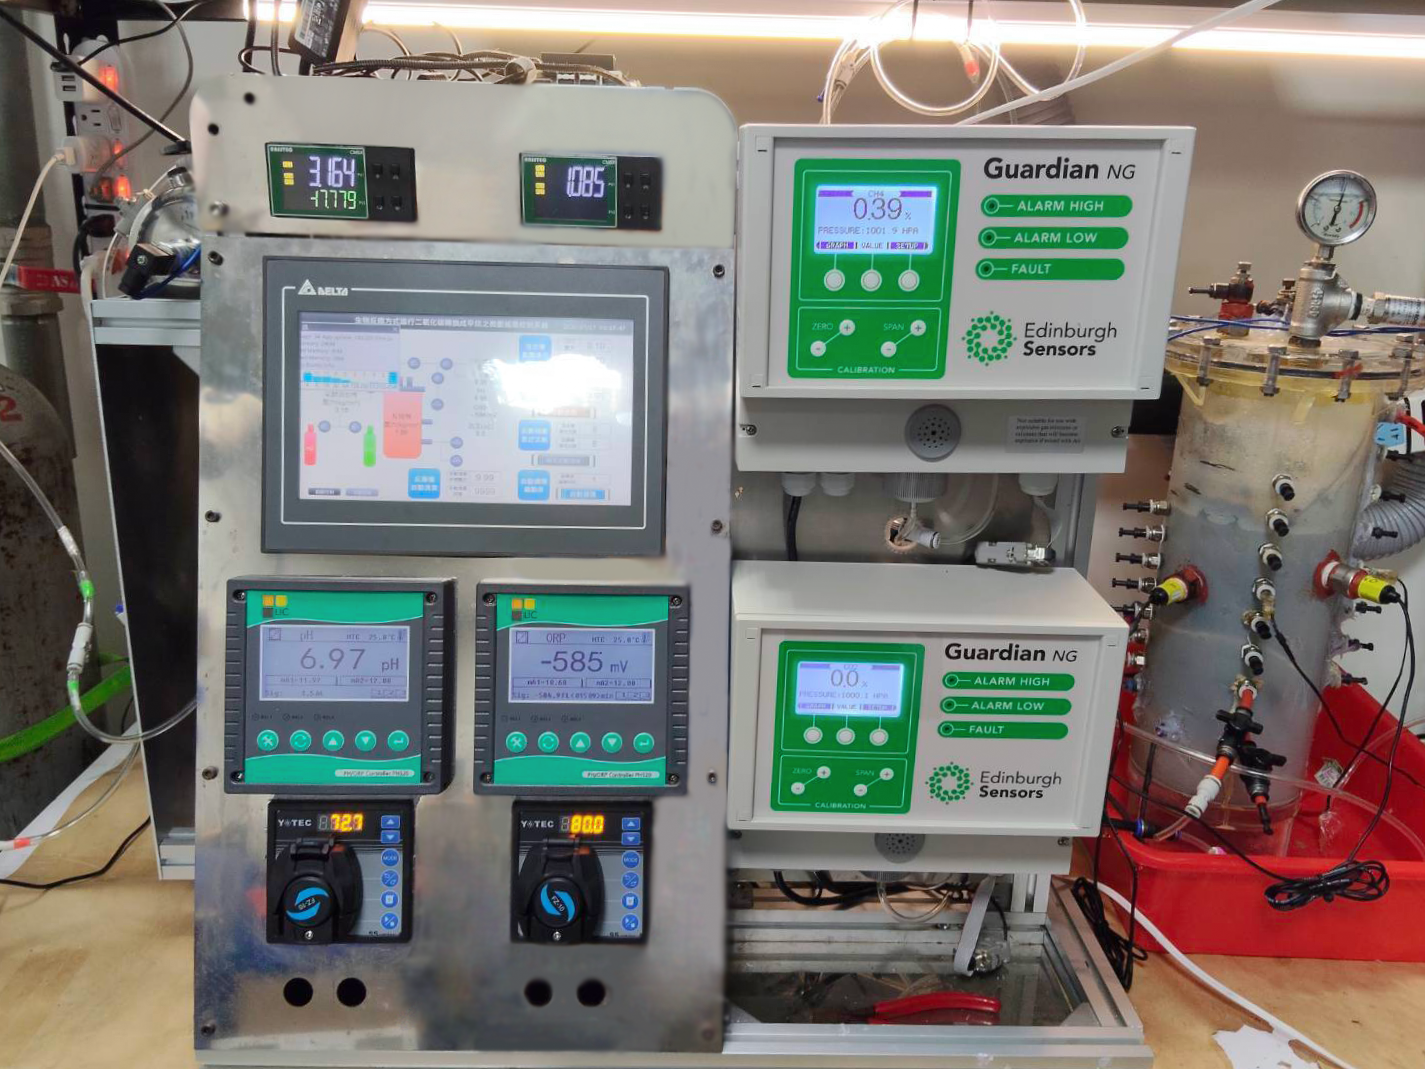
\includegraphics[width=\textwidth]{equipment.png}
\caption{The instrument as built. The panel carries the touch-screen
controller running the plant program, the pH and oxidation--reduction
potential (ORP) meters, and the two optical gas analysers reading
\ce{CH4} and \ce{CO2}; the reactor vessel is at the right. The
pressure record analysed in this paper comes from a transducer in the
headspace of that vessel.}
\label{fig:panel}
\end{figure}

\begin{figure}[t]
\centering

\includegraphics[width=\linewidth]{figE_cascade_narrow.pdf}
\caption{The cascaded pressure-tier design of the reactor. Gas is
stepped down from the reactant tier through the culture tier to the
product tier, so that the culture is held under a small positive
pressure while the analyser downstream stays near ambient. The
recirculation pump returns headspace gas to the bottom of the vessel
as bubbles, which is what keeps the reactant gases dissolving. The
pressure transducer (PT) marked in the headspace is the only channel
this paper uses; the controller that opens valve V3 is a closed unit
whose state is never logged.}
\label{fig:cascade}
\end{figure}

The reactor is a micro-pressurized recirculating vessel operated under
a granted invention patent (TW~I923176). Liquid is recirculated
continuously; the headspace is charged with an \ce{H2}:\ce{CO2} mixture
premixed at $4{:}1$, the stoichiometric ratio for
$\mathrm{CO_2}+4\mathrm{H_2}\rightarrow\mathrm{CH_4}+2\mathrm{H_2O}$.
The controller opens the inlet valve when headspace pressure falls
below a threshold and closes it on reaching a target, so a refill is
complete within about one minute and is treated here as instantaneous.
The arrangement is that of Fig.~\ref{fig:cascade}; the controller reads
pressure and commands the inlet valve, but its state is never logged.

Of the logged channels only four are trustworthy: two pressure
transducers, ORP, and pH. The gas-analyzer
composition channels are stale for $99.98\%$ of samples and are not
used as evidence anywhere in this paper. The present analysis uses the
headspace pressure channel alone.

\begin{figure}[t]
\centering

\includegraphics[width=\textwidth]{figD_device_pipeline.pdf}
\caption{Four days of measured pressure; red lines mark
threshold-triggered refills, about twice a day and $280$ times in
total. Each descending flank is one endogenous relaxation experiment,
and the sawtooth is the signature of the trigger loop.}
\label{fig:device}
\end{figure}

Figure~\ref{fig:device} shows a representative four-day window. Because a refill raises
pressure by far more than the sensor quantum within a single sample
interval, cycle boundaries need no changepoint machinery: a threshold
rule on the rise above the running minimum yields $280$ cycles.

Those cycles are long and shallow. Pressure is logged once a minute, so
a cycle of median duration $10.3$~hr carries roughly $620$ samples. The
median descent amplitude is $0.31$~\pu{}, which is $31$ quantization
steps, while the median residual scale about a fitted trajectory is
$0.0065$~\pu{}, below a single step. The biological term accounts for
roughly half of the descent, so the quantity to be recovered spans on
the order of fifteen steps against a per-sample noise smaller than one.
That is the regime the rest of the paper works in: many samples, a
coarse ladder, and an effect large against the noise but small against
the physical term it must be separated from.

\subsection{Physical and Biological Contributions}

The difficulty runs deeper than the missing channel. A single
relaxation is not enough to separate the two contributions even in
principle. Writing the descent as
\begin{equation}
P(t)=P_{eq}+A\,e^{-kt}-\rb\,t ,
\label{eq:le}
\end{equation}
where $P_{eq}$ is the pressure the headspace would settle at on physics
alone, $A=P(0)-P_{eq}$ is how far the refill leaves it from that value,
and $k$ sets how fast it returns. Table~\ref{tab:params} collects the
four quantities. The exponential term carries the physical approach to
equilibrium and the linear term the constant-rate biological removal,
and the only feature that tells them apart is the curvature of the
exponential.

\begin{table}[t]
\caption{The four quantities of Eq.~\eqref{eq:le}. Only \rb{} is the
target of this paper; the other three describe the physical transient
that has to be separated from it.}
\label{tab:params}
\centering
\begin{tabular}{ll}
\toprule
Symbol & Meaning \\
\midrule
$P_{eq}$ & Physical equilibrium baseline of the headspace \\
$A$      & Initial amplitude of the physical relaxation \\
$k$      & Physical relaxation rate \\
\rb{}    & Biological removal rate \\
\bottomrule
\end{tabular}
\end{table}

Over a window in which $kT$ is small that curvature is never expressed.
Expanding $e^{-kt}\approx 1-kt$ and collecting terms turns
Eq.~\eqref{eq:le} into
\begin{equation}
P(t)\;\approx\;(P_{eq}+A)\;-\;(Ak+\rb)\,t ,
\label{eq:degen}
\end{equation}
a straight line whose slope is the \emph{sum} $Ak+\rb$. A descent of
five units an hour is then explained equally well by $Ak=4$ with
$\rb=1$, by $Ak=2$ with $\rb=3$, or by $Ak=0$ with $\rb=5$: the record
fixes the sum and says nothing about the split. Recovering $\rb$ from
that sum is the problem this paper addresses. Practical
identifiability of exactly this kind
is a recognized open problem in the anaerobic-digestion modeling
literature \cite{donosobravo2011model}, and it persists in the
mechanistic models written specifically for biomethanation: recent
extensions of Anaerobic Digestion Model No.~1 (ADM1) to this process
carry biological and mass-transfer
parameters that must be identified together from the same measurements
\cite{acostapavas2023dynamic}.

Given only the observed pressure trajectory $P(t)$, the objective of
this paper is to estimate \rb{} reliably while separating the transient
physical contribution characterized by $k$. Sections~\ref{sec:method}
and~\ref{sec:results} address, in turn, how that estimate is formed and
how far it can be trusted.

\section{Related Work}
\label{sec:related}

Three lines of work bear directly on this problem, and the first is the
one that most constrains what we may claim.

\subsubsection{Two rates from one gas trace.}
The estimation geometry we face is fifty-nine years old. The dynamic
gassing-out method \cite{bandyopadhyay1967dynamic} extracts, from a
\emph{single} dissolved-gas trace across an interruption of aeration,
both a mass-transfer coefficient and a biological uptake rate: one
scalar channel, one transfer term, one biological term. We inherit that
structure and claim no novelty in it. The regime differs: their
protocol imposes the interruption where ours may not perturb a
production vessel, and they report a point estimate where we report a
degeneracy-calibrated aggregate. Dynamic pressure variants
\cite{linek1989dynamic} likewise rely on an imposed step and treat the
biological term as negligible or independently known.

\subsubsection{Adding a channel rather than resolving the degeneracy.}
Where the split matters in practice, the field measures something else:
manometric biomethane-potential assays separate leakage from conversion
by weighing the bottle \cite{hafner2018quantification}, a second and
physically independent observable. That is why the degeneracy is rarely confronted directly. Where a
quantity cannot be instrumented at all, the field increasingly infers
it from the measurements already available
\cite{rutland2025application}; ours is of that kind, but without
labelled data to learn from, and without the option of a second
channel the identifiability question is unavoidable.

\subsubsection{Identifiability diagnostics.}
The standard diagnostic is the profile likelihood
\cite{raue2009structural}, recently reviewed together with what
identifiability implies for estimation and prediction
\cite{simpson2026parameter}; the ill-conditioning of exponential
fitting was characterized by Varah \cite{varah1985fitting}. Both are
computed \emph{from} a fit, which is the gap our screen addresses: we
must decide which cycles are worth fitting before we have a fit to
diagnose.

\section{Proposed Method}
\label{sec:method}

The method has one estimator and two validations, and it is worth
separating them at the outset. Algorithm~1 is what produces a number:
it screens a cycle and, if the cycle survives, returns $k$ and \rb{}.
Algorithms~2 and~3 produce no estimate of their own; they exist to
answer two questions about the number Algorithm~1 gives---how much of
it is an artifact of the estimator, and whether physics alone could
have produced it. Figure~\ref{fig:method} places the three in that
relation.

Segmentation splits wherever pressure rises more than $0.03$~\pu{}
above the running minimum; segments shorter than $4$~hr or shallower
than $0.10$~\pu{} are discarded, and the first $3$~min of each is
removed because the refill is treated as instantaneous. Cleaning
removes two contaminants that the equipment operators identified:
pipe-washing days, on which the vessel is cycled repeatedly to clean
lines, and the refill interval itself.

The form of \eqref{eq:le} follows from where each process acts.
Methanogens consume gas that is already dissolved, so the headspace
loses gas only across the interface. Just after a refill the liquid is
undersaturated and transfer is fast, which gives the exponential
relaxation $A\,e^{-kt}$; once the liquid is near saturation, transfer
only replaces what the culture removes, and the headspace then drains
at a rate set by the biology, which gives the linear term $-\rb t$.
Treating the two as additive, rather than coupling the biological sink
to the headspace, is what leaves \rb{} identifiable: in the coupled
form $\dot{P}=-k(P-P_{eq})-\rb$ the rate enters only through the
combination $P_{eq}-\rb/k$ and is absorbed by the equilibrium
pressure. Empirically, \eqref{eq:le} wins on $78.1\%$ of cycles by the Akaike information
criterion (AIC)
against pure-linear and pure-exponential alternatives.

Its degeneracy is not a defect of our implementation but a property of
exponential fitting understood since Lanczos and quantified by
Varah \cite{varah1985fitting}; in the language of
Gutenkunst et al.~\cite{gutenkunst2007universally} the model is sloppy
along the direction that trades $A$ and $k$ against \rb{}. On real data
two fits differing by a factor of $2.5$ in \rb{} lie within $1\%$ of the
same residual sum of squares.

\begin{figure}[t]
\centering

\includegraphics[width=\linewidth]{figF_method_flow.pdf}
\caption{The method. Algorithm~1 is the only step that produces a
number: it screens each descent and, for those retained, returns the
pair $(\rbh,\kh)$. Those same estimates are then put to two
independent questions. Algorithm~2 asks how much of the number the
estimator itself introduced, and Algorithm~3 asks whether physics with
no biological term could have produced it. The two answers together
bound what the calibrated rate means.}
\label{fig:method}
\end{figure}

\subsection{Cycle-Level Rate Estimation}

The profile likelihood \cite{raue2009structural} would diagnose this
degeneracy, but it is computed \emph{from} a fit, and on this data a
fit is exactly what we do not yet trust. We therefore screen on the
shape of the raw trajectory before fitting anything.

The screen statistic is the normalized mid-point curvature
\begin{equation}
c \;=\; \frac{y(0)-y(T/2)}{y(0)-y(T)} ,
\label{eq:curv}
\end{equation}
which equals exactly $0.5$ for a straight descent, where the two terms
of \eqref{eq:le} are indistinguishable, and rises as the trajectory
bends. A cycle is retained when $c \ge c^{*}$, with $c^{*}=0.45$ fixed
by recovery on synthetic cycles of known truth $\rb=0.012$: below that
value the recovered median is biased by more than $25\%$.

For a cycle that survives the screen, Eq.~\eqref{eq:le} is non-linear
in $k$ alone: once $k$ is held fixed the model is linear in $A$,
$P_{eq}$ and \rb{}. Writing the design matrix for a candidate $k$ as
\begin{equation}
D(k)=\left[\,e^{-kt},\; t,\; \mathbf{1}\,\right] ,
\label{eq:design}
\end{equation}
the remaining three coefficients follow in closed form from ordinary
least squares, $\hat{\boldsymbol\beta}(k)=\arg\min_{\boldsymbol\beta}
\lVert y-D(k)\boldsymbol\beta\rVert^{2}$, with residual
\begin{equation}
S(k)=\bigl\lVert y-D(k)\,\hat{\boldsymbol\beta}(k)\bigr\rVert^{2} ,
\qquad
\hat{k}=\arg\min_{k\in K} S(k) .
\label{eq:profile}
\end{equation}
The four-parameter non-linear fit therefore reduces to a scan over a
grid $K$ of $150$ values with one exact $3\times3$ solve at each,
and \rbh{} is read off as the negative of the coefficient on $t$ at
$\hat{k}$. Profiling is preferred to a joint non-linear optimiser for
reasons beyond speed. The scan is exhaustive over $K$, so the minimum
reported is global on that grid and no starting value has to be
guessed---which matters precisely here, because
Eq.~\eqref{eq:degen} makes the objective nearly flat and a descent
method can halt anywhere along it while reporting convergence. The
profile is also its own diagnostic: where the degeneracy bites, $S(k)$
has no distinct minimum, so the curve that yields $\hat{k}$ shows at
the same time how weakly the data constrain it.
Eq.~\eqref{eq:curv} is the cheaper test that anticipates this before
any fit is run. Algorithm~1 states the screen and this estimator together;
both run in NumPy alone, within the $60$~MB budget of the monitoring
computer.

\begin{figure}[t]
\noindent\textbf{Algorithm 1  Extracting a Trustworthy Rate from One Cycle} Cycles too straight to constrain the relaxation constant are rejected before any fit is attempted. The profiled
least-squares estimator for \eqref{eq:le}. Solving all $150$ grid
values of $k$ as one stacked $3\times3$ system keeps a full pass over
$280$ cycles under one second

\begin{verbatim}
Input: one cycle (t, y) of duration T
Parameter: c* = 0.45, grid K over k
Output: the estimates r_b and k for the cycle
c <- (y(0)-y(T/2)) / (y(0)-y(T))  // shape only
if c < c* then reject the cycle and stop
for each k in K do
    D(k) <- [exp(-k t), t, 1]     // design matrix
    b(k) <- argmin_v |y - D(k)v|^2  // 3x3 solve
    s(k) <- |y - D(k) b(k)|^2     // residual
end for
k_fit <- argmin_k s(k)
return r_b = -b_2(k_fit) and k_fit
\end{verbatim}

\end{figure}

Line~1 computes the curvature
$c$ of Eq.~\eqref{eq:curv} from three points of the raw trajectory; no
model is fitted, so nothing about a fit can influence what follows.
Line~2 discards the cycle outright when $c$ falls below $c^{*}$: such a
descent is too straight for the two terms of Eq.~\eqref{eq:le} to be
told apart, and no estimate is preferable to a meaningless one.
Line~3 opens a sweep over the grid $K$, which is worth doing because
Eq.~\eqref{eq:le} is linear in $P_{eq}$, $A$ and \rb{} once $k$ is
held fixed. Line~4 builds the design matrix for the current $k$,
Line~5 solves the resulting $3\times3$ least-squares problem in closed
form, and Line~6 records its residual sum of squares. Line~7 closes
the sweep, which has by then replaced one four-parameter non-linear
fit with $150$ exact linear ones---the reason a full pass stays inside
the memory budget of the monitoring computer. Line~8 keeps the $k$
whose residual was smallest, and Line~9 returns it together with
\rb{}, read off as the negative of the coefficient on $t$ because the
linear term enters Eq.~\eqref{eq:le} with a minus sign.

\subsection{Parameter-Degeneracy Assessment}

Across the retained cycles the fitted \rbh{} and \kh{} correlate at
$\rho=0.814$, which read naively looks like proof that the estimate is
an artifact. It is not readable in isolation: \rbh{} and \kh{} jointly
absorb the same descent, so they correlate even when the truth is
fixed. The question is how far the correlation \emph{exceeds} what a
fixed truth already produces.

We therefore apply empirical calibration in the sense of Schuemie et
al.~\cite{schuemie2014interpreting}, replacing the theoretical null
$\rho=0$ with one estimated from cases where the truth is known. The
null is generated by design-matched simulation (Algorithm~2): each real
cycle contributes its own fitted $\kh,\hat{A},\hat{P}_{eq}$, duration,
residual scale and first-order autoregressive
(AR(1)) coefficient, only the true \rb{} is
substituted, and the result passes through the identical pipeline, so
the estimator's distortion appears on both sides and cancels---the
logic of indirect inference \cite{gourieroux1993indirect}. Our adaptation is the source of the negative controls: ours are
simulations reusing the real designs, which fixes the truth exactly
instead of assuming it.

\begin{figure}[t]
\noindent\textbf{Algorithm 2  Measuring and Removing the Degeneracy Bias} Sweeping
$\beta$ with this routine gives the curve of Fig.~\ref{fig:matched};
a constant truth ($\beta=0$) returns $\rho=0.304\pm0.056$, and a truth
independent of $k$ returns $\rho=0.143\pm0.048$, against an observed
$0.814$

\begin{verbatim}
Input: per-cycle fits k, A, P_eq, t, sigma, phi
Parameter: truth r_b(.), R = 25, quantum q = 0.01
Output: baseline distributions of rho and m
for r <- 1 to R do
  for i <- 1 to 239 do
    e <- AR(1) noise, 1.3 phi, scale sigma
    z <- P_eq + A exp(-k t) - r_b(k) t + e
    y <- q round(z / q)         // same quantum
    (rb, kk) <- Algorithm 1 (t, y)
  end for
  rho(r) <- Spearman(rb, kk)    // over the 239
  m(r) <- median(rb)
end for
return the distributions of rho and m
\end{verbatim}

\end{figure}

Line~1 repeats the whole
pipeline $R$ times, so that the baseline comes out as a distribution
rather than a single number, and Line~2 walks the $239$ retained
cycles inside each repetition. Line~3 draws the noise as AR(1) at
that cycle's own residual scale rather than as white noise, because
the measured residuals are not white. Line~4 assembles the synthetic
trace from that same cycle's own fitted $P_{eq}$, $A$ and $k$, with
only the biological rate replaced by the candidate truth $\rb(k)$:
every quantity except the one under test is inherited from the real
cycle, so the distortion measured is the distortion that applies to
\emph{that} cycle. Line~5 puts the trace through the same
$0.01$~\pu{} quantization as the instrument, and Line~6 through the
estimator of Algorithm~1, unchanged. Line~7 closes the pass over the
cycles. Line~8 then records the correlation the pipeline produces
from a truth that is known, which is the quantity to be compared
against the observed $\rho$, and Line~9 records the aggregate median,
whose departure from the truth put in is the bias to be removed.
Line~10 closes the repetitions and Line~11 returns both
distributions.

The simulator itself must be shown adequate, or the baseline means
nothing. We use a classifier two-sample test, introduced for this
purpose by Friedman \cite{friedman2003multivariate} and revisited by
Lopez-Paz and Oquab \cite{lopezpaz2017revisiting}, and applied to
simulator and emulator validation by Dalmasso et
al.~\cite{dalmasso2020validation}: a classifier is trained to tell real
trajectories from simulated ones, and an area under the receiver
operating characteristic curve (AUC) near $0.5$ indicates the
two are indistinguishable. The noise model is calibrated on one half of
the cycles and the AUC computed on the held-out half.

\subsection{Purely Physical Null-Model Test}
\label{sec:null}

The validity of the test behind $p=0.024$ (Algorithm~3) rests on what the null is
allowed to contain. For each retained cycle we fit the two-parameter
form $P(t)=P_{eq}+A\,e^{-kt}$, that is \eqref{eq:le} with $\rb$ forced
to zero, so the fitted null reproduces the cycle's own equilibrium,
amplitude and relaxation constant. We regenerate the cycle from that
fit, add AR(1) noise at its own residual scale, quantize to
$0.01$~\pu{}, and pass it through the identical screen and estimator.
Over all $239$ cycles this yields one draw of the aggregate median
under a physics-only truth; $60$ draws give its null distribution.

\begin{figure}[t]
\noindent\textbf{Algorithm 3  Ruling Out a Purely Physical Explanation}
The reference is fitted per cycle, so it inherits every degree of
freedom the alternative has except the biological rate itself, and it
passes through the same quantization, screen and estimator

\begin{verbatim}
Input: the retained cycles (t, y), i = 1..239
Parameter: draws D, grid K, quantum q = 0.01
Output: reference distribution of the median
for i <- 1 to 239 do
  fit P_eq + A exp(-k t) to (t, y)  // r_b = 0
  sigma <- residual scale of that fit
end for
for d <- 1 to D do
  for i <- 1 to 239 do
    e <- AR(1) noise at scale sigma
    z <- P_eq + A exp(-k t) + e
    w <- q round(z / q)         // same quantum
    rb <- Algorithm 1 (t, w)    // same estimator
  end for
  m(d) <- median(rb)
end for
return the distribution of m over D draws
\end{verbatim}

\end{figure}

Lines~1 to~4
construct the reference. Line~2 refits each cycle with the rate
forced to zero, so the resulting $P_{eq}$, $A$ and $k$ are the best
purely physical account of that particular descent, and Line~3 keeps
the residual scale of that fit so the synthetic noise matches what
physics alone leaves behind; Line~4 closes the pass. Line~5 then
draws $D$ realisations of the reference and Line~6 walks the cycles
within each. Line~7 draws AR(1) noise at the scale just recorded and
Line~8 generates a trace from the physics-only fit, with no linear
term present at all. Line~9 applies the same quantization and
Line~10 the same estimator, which is what makes the outcome
interpretable: any rate reported here is an artifact of the pipeline,
since there is no biological rate in the data to find. Line~11 closes
the pass over cycles, Line~12 records the aggregate median of that
realisation, Line~13 closes the draws, and Line~14 returns the
resulting distribution.

The null is fitted per cycle rather than pooled, so it is granted every
degree of freedom the alternative has except $\rb$ itself. Under it the
aggregate median is
$+0.00008 \pm 0.00010$~\ratu{}, two orders of magnitude below the
observed $0.0128$.

\section{Experimental Results}
\label{sec:results}

The results are organised by question rather than by algorithm: which
cycles enter the analysis, what rate they give, how much of that rate
survives the degeneracy, whether physics alone can account for it, and
whether an independent channel agrees.

\subsection{Experimental Setup and Pressure Cycles}
\label{sec:setup}

The record analysed here is the plant's own operating log: one pressure
value a minute, quantized at $0.01$~\pu{}, with nothing added to the
instrument and no excitation imposed on it. Applying the threshold rule
of Sect.~\ref{sec:dynamics} to the whole archive segments $351$
descents, logged over periods that do not all share the same operating
condition, and three groups are set aside before any rate is compared.
One period was charged at an \ce{H2}:\ce{CO2} ratio of $1{:}1$ instead
of the $4{:}1$ of Sect.~\ref{sec:dynamics}, which changes the
proportion in which the two gases leave the headspace. One covers an
interval during which liquid recirculation was switched off, so
gas--liquid transfer is not the regime Eq.~\eqref{eq:le} describes.
The third returns a negative median rate---biology producing
pressure---which is physically impossible and points to a fault in the
record rather than to a slow culture.

The first two criteria are settled by the recorded operating condition
alone. The third is not: it is settled by the fitted result, and we
therefore report what happens without it. Keeping only the two
condition-based exclusions moves the screened median from $0.0128$ to
$0.0124$~\ratu{}, and applying none of the three moves it to
$0.0117$~\ratu{}; the two shifts, $-3.5\%$ and $-8.6\%$, are both
smaller than the accuracy quoted for the reported rate, so the result
does not rest on the exclusion that looked at an outcome. What the
exclusions leave is $280$ cycles, of which the curvature screen retains
$239$. The median descent runs for $10.3$~hr, with quartiles at $6.9$
and $22.5$~hr.

Those $239$ cycles come from five logging periods whose individual
medians run from $0.0074$ to $0.0203$~\ratu{}, and dropping either of
the two largest periods moves the aggregate by $-11.3\%$ or $+20.6\%$.
That spread is wider than the $\pm 11.9\%$ attached to
Eq.~\eqref{eq:rate}, and the two statements do not contradict each
other: the interval says how precisely the median of \emph{this} record
is pinned down, not how steady the culture is from month to month. The
rate reported below is an aggregate over the record analysed, and the
variation between periods is itself what
Sect.~\ref{sec:degen} establishes on independent grounds---a rate that
is constant across cycles is excluded by the calibration.

\subsection{Physical and Biological Rate Estimation}

Figure~\ref{fig:estimates} shows what Algorithm~1 returns on the
retained cycles.
Panel~(a) is a single cycle whose $\hat{k}$ and \rbh{} both sit close
to the medians of the retained set: the fitted trajectory follows the
quantized record over ten hours, and the gap between the fitted total
and its physical part is the biological contribution the decomposition
is there to isolate. Panels~(b) and~(c) give the distributions over all
retained cycles. The relaxation constant spans two orders of magnitude
with median $0.15$~\invh{}, and the per-cycle rate has median
$0.0128$~\ratu{} before calibration.

\begin{figure*}[t]
\centering

\includegraphics[width=\textwidth]{figG_estimates.pdf}
\caption{What the estimator returns on the $239$ retained cycles.
(a)~A cycle with \kh{} and \rbh{} near the medians of the set; the
logged trace advances in steps of $0.01$~\pu{}, and the shaded band
between the fitted total and its physical part is the biological
contribution. (b)~Distribution of the fitted relaxation
constant, on a logarithmic axis. (c)~Distribution of the fitted
biological rate; the dotted line marks zero, and values outside the
plotted range are collected in the end bars rather than shown at their
own positions.}
\label{fig:estimates}
\end{figure*}

The spread in panel~(c) is why the aggregate is reported and the
per-cycle value is not: $50$ of the $239$ cycles return a negative
rate, which is physically impossible and is the degeneracy of
Sect.~\ref{sec:dynamics} expressing itself on individual descents.

That spread also fixes how the cycles are pooled. With those negative
values at one end and a tail reaching several times the centre at the
other, the mean over per-cycle estimates is neither robust nor
interpretable, whereas the median of a set whose members are noisy but
not systematically ordered remains a usable summary. The median is
equally what the calibration is built around: the matched simulations
of Sect.~\ref{sec:degen} report that same functional on data generated
from a known truth, so the distortion measured there is the distortion
of the quantity actually reported. The estimand is therefore the median
rate over the cycles the screen retains, and every correction and
interval quoted below refers to that functional rather than to any
individual cycle. What the median survives and a single cycle does not
is the subject of the next two subsections.

\subsection{Robustness Against Parameter Degeneracy}
\label{sec:degen}

Rather than assume a form for the $k$ dependence, we treat its strength
as the quantity to be inverted. Writing the truth as
$\rb(k)=\rb^{0}(k/k_{med})^{\beta}$---a power law, so that \rb{} cannot
turn negative and the median truth is $\rb^{0}$ for every
$\beta$---we sweep $\beta$ and run the full matched pipeline at each
value, obtaining the calibration curve of Fig.~\ref{fig:matched}(a).

\begin{table}[t]
\caption{The recovered rate and the calibration checks behind it. The
baseline rows are design-matched simulations in which the true rate is
known, so the estimator's own distortion can be read off directly.}
\label{tab:rate}
\centering
\begin{tabular}{lrr}
\toprule
Quantity & Value & Note \\
\midrule
Descents segmented & $351$ & threshold rule \\
Cycles analysed & $280$ & after condition exclusions \\
Cycles retained & $239$ & $c \ge 0.45$ \\
Calibrated \rb{} & $0.0126$~\ratu{} & $95\%$ $[0.0112,\ 0.0142]$ \\
\quad sampling component & $\pm 5.5\%$ & bootstrap over $239$ cycles \\
\quad systematic component & $\pm 5.1\%$ & over the compatible set \\
Physics-only reference & $p=0.024$ & pure exponential truth \\
\midrule
Observed $\rho(\rbh,\kh)$ & $0.814$ & \\
Calibration, $\beta=0$ (constant) & $0.304 \pm 0.056$ & artefact level \\
Baseline, \rb{} independent of $k$ & $0.143 \pm 0.048$ & \\
Compatible set & $0.20 \le \beta \le 0.80$ & within calibration scatter \\
\midrule
Raw profiled median & $0.0128$~\ratu{} & before correction \\
Calibrated correction & $-3.7\%$ & estimator distortion only \\
\bottomrule
\end{tabular}
\end{table}

A constant truth is excluded: $\beta=0$ produces only
$\rho=0.304 \pm 0.056$ against the observed $0.814$, a gap of roughly
nine standard deviations, and making \rb{} merely variable without
tying it to $k$ lowers the correlation further, to $0.143$. Truths
with $\beta$ between $0.20$ and $0.80$ reproduce the observed
correlation to within the calibration scatter, and it is that
compatible set we carry forward.

The same calibration then supplies the correction
(Fig.~\ref{fig:matched}(b)), and it separates two effects that must not
be conflated. The screen admits cycles by curvature, so the truths it
keeps are not those of the whole population; that displacement grows
with $\beta$ and reaches $37\%$ at the top of the compatible set. It is
not an error but a definition: we report the rate \emph{on the cycles
where it is identifiable}, and the screen is what makes them so. What
must be corrected is the estimator's own distortion, measured against
the truths actually kept, and that stays between $-4.1\%$ and $+5.8\%$
across the whole compatible set. Inverting it corrects the raw
profiled median by $-3.7\%$, to $0.0124$~\ratu{}, at the centre of the
compatible set. That single point is not the reported value. Because
the correction enters as a quotient and the bias is not symmetric
across the set, we draw the bias and the sampling error together by
Monte Carlo, which shifts the centre slightly and gives the calibrated
rate
\begin{equation}
\rb = 0.0126\ [0.0112,\ 0.0142]~\ratu{} .
\label{eq:rate}
\end{equation}

The interval combines two sources that behave differently. Resampling
the $239$ cycles gives $\pm 5.5\%$ on the median, which shrinks as
logging continues; the spread over the compatible truths is
$\pm 5.1\%$ and does not, being set by how sharply the calibration
separates members of the family rather than by how many cycles are
seen. Since the correction enters as a quotient we draw from both by
Monte Carlo, giving the $\pm 11.9\%$ of \eqref{eq:rate}---the accuracy
with which a single quantized pressure channel fixes the biological
rate, and the main quantitative result of this paper.

The classifier two-sample test is reported next. A
white-Gaussian noise model is separated at $\mathrm{AUC}=0.968$; the
residuals of real cycles in fact carry a lag-1 autocorrelation with
median $0.266$. Modeling the noise as AR(1) reduces this to $0.832$,
and inflating $\hat{\varphi}$ by the factor $1.3$ calibrated on the
held-out split reaches $0.695$. All ten marginal trajectory features
then agree to within $0.29$ pooled standard deviations, the largest gap
being the monotone fraction ($0.808$ against $0.786$), with curvature,
residual scale, lag-1 autocorrelation, amplitude and duration all
within $0.15$; we return to the residual mismatch in
Sect.~\ref{sec:limits}.

\label{sec:endpoint}

Segmentation ends each cycle at the sample immediately before a refill,
and that sample is selected \emph{because} pressure fell far enough to
trigger, so it sits below the underlying trend: stacked residuals give
a terminal mean of $-0.068$ of the cycle amplitude against $\pm 0.006$
elsewhere. Since a linear slope is most sensitive at its endpoints,
this is a plausible route to an inflated rate.

Trimming settles it. Removing the last $5$ to $90$ minutes of every
cycle moves the median \rb{} only within $0.0124$--$0.0133$~\ratu{}, a
band of $\pm 5\%$, and a design-matched simulation with no trigger
selection drifts comparably: one anomalous sample among roughly $620$
has too little leverage to bend the slope.

\begin{figure}[t]
\centering

\includegraphics[width=\linewidth]{figB_matched_baseline.pdf}
\caption{(a) Calibration of the correlation against the strength
$\beta$ of the $k$ dependence, each point a full matched pipeline; the
band is $\pm1$ standard deviation over repetitions and the shaded
region is the compatible set. A constant truth ($\beta=0$) falls nine
standard deviations below the observation. (b) The bias read from the
same calibration: the estimator's own distortion, which is what we
correct, and the screen's selection of truths, which is definitional;
inverting it yields the $-3.7\%$ correction applied to the rate.}
\label{fig:matched}
\end{figure}

\subsection{Evaluation Against the Purely Physical Null Model}

The remaining question is whether the observed rate could have arisen
with no biology at all. Following Algorithm~3, each retained cycle is
refitted with \rb{} forced to zero, regenerated from that fit with
AR(1) noise at its own residual scale, quantized to $0.01$~\pu{}, and
passed through the same screen and the same estimator. The reference
therefore keeps every degree of freedom the alternative has except the
biological term itself.

\begin{figure}[t]
\centering

\includegraphics[width=\textwidth]{figH_null.pdf}
\caption{The physics-only reference never reaches the observed rate.
Bars are the aggregate median returned by the same pipeline when the
truth is $\rb\equiv 0$; the vertical line is the observed median.}
\label{fig:null}
\end{figure}

The reference does not come close. Its aggregate median is
$0.00038$~\ratu{} and its largest draw reaches $0.0026$, against an
observed median of $0.0128$: no draw attains the observation, which
gives a permutation $p=0.024$ over $41$ draws
(Fig.~\ref{fig:null}). The pressure descent therefore contains a
component that a physics-only model cannot produce. We stress the
direction of this inference: it excludes a purely physical explanation;
it does not by itself establish that the residual component is
biological.

\subsection{An Independent Check from Redox Potential}

Everything above is derived from pressure, and surviving a
physics-only reference says what the residual component cannot be, not
what it is. The reactor also logs ORP. It
enters no part of the estimate and is not a rate. Redox potential is an
established monitoring variable for anaerobic digestion, used as an
indicator of process state and as an early warning of instability
\cite{ao2021role}, with methanogenesis reported to proceed in a
characteristic reducing window \cite{vongvichiankul2017relationship};
the potential recorded here, referred to the standard hydrogen
electrode, falls inside that window. It is a mixed potential rather
than a probe of any single species, so we use it only to order cycles,
never to measure a rate, and that is what makes it usable as a check.

Sorting the cycles by the net change in redox potential across each
cycle and comparing the aggregate rate across terciles gives $0.0099$,
$0.0134$ and $0.0152$~\ratu{} from least to most active, a $54\%$ span
whose bootstrap interval, $[0.0004,\ 0.0137]$, excludes zero. Because
that change is taken over the whole cycle it is partly confounded with
cycle duration: the rank correlation with $\rb$ falls from $0.21$ to
$0.15$ when duration is controlled for, but does not vanish. A quantity
measured on a different physical channel, in the liquid rather than the
gas, therefore orders the same rates that the pressure trajectories
give.

The ordering is aggregate rather than per cycle, and what it
establishes is that the variation the calibration detected in $\rb$
tracks an independently measured signature of biological activity,
which pressure alone could not have shown.

\section{Discussion}
\label{sec:limits}

\subsubsection{Why pressure decline cannot be read as biological
activity.}
The pressure record is cheap, continuous and already being logged,
which is what makes it attractive for process monitoring; the
difficulty is that a descent is not a measurement of the culture. Every
refill leaves the liquid undersaturated, so for part of each cycle the
headspace is losing gas to dissolution at the same time as the culture
is consuming it. Reading the descent rate as biological activity
therefore overstates it, and the overstatement is largest exactly when
the plant has just been refilled. That is the reason the decomposition
of Eq.~\eqref{eq:le} is needed at all, and the reason a screen has to
run before the fit: on a cycle whose curvature is too weak, the two
contributions are interchangeable and no fit can apportion them.

\subsubsection{What the recovered rate is, and what it is not.}
The quantity in Eq.~\eqref{eq:rate} is a \emph{pressure-derived
biological removal rate}: the part of the headspace pressure loss that
a purely physical model cannot produce. It is not a methane production
rate. Converting one into the other would require the headspace volume
and the operating temperature, and would then have to be checked
against a composition measurement, which this instrument cannot supply
because its analyser channels are stale for $99.98\%$ of samples. The
direction of the inference matters as much as its size: the null test
of Sect.~\ref{sec:null} excludes a purely physical explanation, and
attributing the residual to biology rests on the redox ordering and on
the stoichiometry of the process, not on the pressure channel itself.
Used as a relative indicator on one vessel over time---has the rate
fallen since last week, did the new circulation setting help---the
number is on firmer ground than it would be as an absolute figure.

\subsubsection{Limitations.}
Three limits bound what the preceding numbers support. First,
Eq.~\eqref{eq:le} treats \rb{} as constant within a cycle. That is a
simplifying assumption: the culture is not obliged to consume at a
fixed rate across ten hours, and a slow decline within the cycle would
be partly absorbed by the exponential term. It is the assumption that
makes the linear term identifiable at all, and relaxing it would
require a second observable.

Second, the aggregate median is recoverable but the per-cycle estimates
are not: individual values scatter widely and are coupled to \kh{}, so
nothing here licenses reading a single cycle as a rate measurement. The
same applies to the redox check: it also responds to pH and to
dissolved carbon dioxide, so it is not a hydrogen probe, and without a
composition anchor it cannot be turned into a rate to set against
Eq.~\eqref{eq:rate}. Of the $\pm 11.9\%$ on the rate, the $\pm 5.1\%$
systematic part is fixed by the calibration rather than by the record
length; narrowing it needs the form of $\rb(k)$ itself, which a second
chemical channel would supply.

Third, the simulator remains distinguishable from reality at
$\mathrm{AUC}=0.695$ even after all ten marginal features are matched,
so the mismatch lies in joint structure we have not identified. The
matched baselines are consequently approximate, and we do not attempt
simulation-based inference on this simulator: a posterior learned from
a misspecified simulator would be narrow and wrong rather than merely
uncertain.

\section{Conclusion}

We have presented a pressure-based framework that separates the
transient physical relaxation following a refill from the sustained
biological gas removal that continues through a biomethanation cycle,
using a single pressure channel quantized at $0.01$~\pu{} and nothing
added to a vessel in production. A screen computed from the raw
trajectory decides which cycles can carry the separation at all, and
the estimator returns a rate only for those.

Two validations bound what that rate means. A design-matched
calibration measures the distortion the estimator itself introduces and
removes it, and in doing so rules out a constant biological rate across
cycles. A purely physical null model, fitted per cycle and passed
through the same screen and estimator, shows that physical relaxation
alone does not reproduce the observed removal. Across $239$ screened
cycles the recovered rate is $0.0126$~\ratu{}, accurate to $11.9\%$, of
which $5.1\%$ is systematic and does not shrink with a longer record.

Future work will validate this pressure-derived biological removal rate
against direct methane-production measurements, which would also fix
the conversion to molar units, and will examine its use as a real-time
indicator of culture activity in continuous biomethanation.

\subsubsection{Acknowledgements.} The reactor is operated under
invention patent TW~I923176 held by the Metal Industries Research \&
Development Centre.

% 13 筆。改版時砍掉 7 筆較邊緣者以省版面：jackson2005／killick2012
% （§3 原本誤述為用最佳分割切分，實際是閾值規則，連同誤述一併移除）、
% scargiali2010（與 linek1989 重複）、pastorpoquet2019（與 donosobravo2011
% 重複）、decrescenzo2022、guerrier2019（與 gourieroux1993 重複）、
% palminteri2017（與 wilson2019 重複）。每一筆保留者都在正文被引用過。

\begin{thebibliography}{12}

\bibitem{acostapavas2023dynamic}
Acosta-Pavas, J.C., Robles-Rodr\'{i}guez, C.E., Morchain, J., Dumas, C.,
Cockx, A., Aceves-Lara, C.A.: Dynamic modeling of biological methanation
for different reactor configurations: an extension of the anaerobic
digestion model No.~1. Fuel \textbf{344}, 128106 (2023)

\bibitem{ao2021role}
Ao, T., Chen, L., Zhou, P., Liu, X., Li, D.: The role of
oxidation--reduction potential as an early warning indicator, and a
microbial instability mechanism in a pilot-scale anaerobic mesophilic
digestion of chicken manure. Renew. Energy \textbf{179}, 223--232 (2021)

\bibitem{bandyopadhyay1967dynamic}
Bandyopadhyay, B., Humphrey, A.E., Taguchi, H.: Dynamic measurement of
the volumetric oxygen transfer coefficient in fermentation systems.
Biotechnol. Bioeng. \textbf{9}(4), 533--544 (1967)

\bibitem{dalmasso2020validation}
Dalmasso, N., Lee, A.B., Izbicki, R., Pospisil, T., Kim, I., Lin,
C.-A.: Validation of approximate likelihood and emulator models for
computationally intensive simulations. In: AISTATS. PMLR, vol.~108,
pp. 3349--3361 (2020)

\bibitem{donosobravo2011model}
Donoso-Bravo, A., Mailier, J., Martin, C., Rodr\'{i}guez, J.,
Aceves-Lara, C.A., Vande Wouwer, A.: Model selection, identification
and validation in anaerobic digestion: a review. Water Res.
\textbf{45}(17), 5347--5364 (2011)

\bibitem{friedman2003multivariate}
Friedman, J.H.: On multivariate goodness-of-fit and two-sample testing.
In: Proc. PHYSTAT2003, SLAC, Stanford, CA. SLAC-PUB-10325 (2003)

\bibitem{ghiat2025circularity}
Ghiat, I., Banu, A., Bicer, Y., Amhamed, A.I., Al-Ansari, T.:
Circularity within carbon capture networks: a review of capture and
utilization technologies. J. CO2 Util. \textbf{95}, 103075 (2025)

\bibitem{gonzalez2023biological}
Gonz\'{a}lez, R., Cabeza, I.O., Casallas-Ojeda, M., G\'{o}mez, X.:
Biological hydrogen methanation with carbon dioxide utilization:
methanation acting as mediator in the hydrogen economy. Environments
\textbf{10}(5), 82 (2023)

\bibitem{gourieroux1993indirect}
Gouri\'{e}roux, C., Monfort, A., Renault, E.: Indirect inference.
J. Appl. Econom. \textbf{8}(S1), S85--S118 (1993)

\bibitem{gugler2023carbon}
Gugler, K., Haxhimusa, A., Liebensteiner, M.: Carbon pricing and
emissions: causal effects of Britain's carbon tax. Energy Econ.
\textbf{121}, 106655 (2023)

\bibitem{gutenkunst2007universally}
Gutenkunst, R.N., Waterfall, J.J., Casey, F.P., Brown, K.S., Myers,
C.R., Sethna, J.P.: Universally sloppy parameter sensitivities in
systems biology models. PLoS Comput. Biol. \textbf{3}(10), e189 (2007)

\bibitem{hafner2018quantification}
Hafner, S.D., Rennuit, C., Olsen, P.J., Pedersen, J.M.: Quantification
of leakage in batch biogas assays. Water Pract. Technol.
\textbf{13}(1), 52--61 (2018)

\bibitem{linek1989dynamic}
Linek, V., Bene\v{s}, P., Vacek, V.: Dynamic pressure method for
$k_{L}a$ measurement in large-scale bioreactors. Biotechnol. Bioeng.
\textbf{33}(11), 1406--1412 (1989)

\bibitem{lopezpaz2017revisiting}
Lopez-Paz, D., Oquab, M.: Revisiting classifier two-sample tests. In:
International Conference on Learning Representations (2017)

\bibitem{raue2009structural}
Raue, A., Kreutz, C., Maiwald, T., Bachmann, J., Schilling, M.,
Klingm\"{u}ller, U., Timmer, J.: Structural and practical
identifiability analysis of partially observed dynamical models by
exploiting the profile likelihood. Bioinformatics \textbf{25}(15),
1923--1929 (2009)

\bibitem{rutland2025application}
Rutland, H., You, J., Liu, H., Bowman, K.: Application of machine learning
for FOS/TAC soft sensing in bio-electrochemical anaerobic digestion.
Molecules \textbf{30}(5), 1092 (2025)

\bibitem{schuemie2014interpreting}
Schuemie, M.J., Ryan, P.B., DuMouchel, W., Suchard, M.A., Madigan, D.:
Interpreting observational studies: why empirical calibration is needed
to correct p-values. Stat. Med. \textbf{33}(2), 209--218 (2014)

\bibitem{simpson2026parameter}
Simpson, M.J., Baker, R.E.: Parameter identifiability, parameter
estimation, and model prediction for differential equation models.
SIAM Rev. \textbf{68}(1), 153--171 (2026)

\bibitem{varah1985fitting}
Varah, J.M.: On fitting exponentials by nonlinear least squares. SIAM
J. Sci. Stat. Comput. \textbf{6}(1), 30--44 (1985)

\bibitem{vongvichiankul2017relationship}
Vongvichiankul, C., Deebao, J., Khongnakorn, W.: Relationship between
pH, oxidation reduction potential (ORP) and biogas production in
mesophilic screw anaerobic digester. Energy Procedia \textbf{138},
877--882 (2017)

\bibitem{yoruklu2025comprehensive}
Y\"{o}r\"{u}kl\"{u}, H.C., Kamravamanesh, D., K\"{o}ro\u{g}lu, E.O.,
Patel, G.H., Havukainen, J., Karjunen, H., Sillman, J., Kokko, M.:
A comprehensive review on biological methanation processes: from gaseous
feedstocks to biomethane. Energy Convers. Manag. \textbf{341}, 120075
(2025)

\end{thebibliography}

\end{document}
